\documentclass[letterpaper, 10 pt, conference]{ieeeconf}

\IEEEoverridecommandlockouts                              % This command is only needed if
   % you want to use the \thanks command

\overrideIEEEmargins                                      % Needed to meet printer requirements.

% See the \addtolength command later in the file to balance the column lengths
% on the last page of the document

% The following packages can be found on http:\\www.ctan.org
\usepackage{graphicx}
%\usepackage{epsfig} % for postscript graphics files
%\usepackage{mathptmx} % assumes new font selection scheme installed
%\usepackage{times} % assumes new font selection scheme installed
%\usepackage{amsmath} % assumes amsmath package installed
%\usepackage{amssymb}  % assumes amsmath package installed
\usepackage[brazilian]{babel}
\usepackage[utf8]{inputenc}
\usepackage[T1]{fontenc}

\title{\LARGE \bf
Reconstrução de modelos 3D para uso na medicina
}


\author{
Marlon Henry Schweigert \& Roberto Silvio Ubertino Rosso
\\Universidade do Estado de Santa Catarina
\\Centro de Ciências Tecnológicas
\\Automação e Controle
}


\begin{document}



\maketitle
\thispagestyle{empty}
\pagestyle{empty}


%%%%%%%%%%%%%%%%%%%%%%%%%%%%%%%%%%%%%%%%%%%%%%%%%%%%%%%%%%%%%%%%%%%%%%%%%%%%%%%%
\begin{abstract}
Este pseudo artigo visa buscar as últimas tecnologias utilizando reconstrução 3D para auxilio médico, visando desempenho e utilização de técnicas que abordam reconstrução 3D a partir de imagens no ambiente hospitalar.
\end{abstract}


%%%%%%%%%%%%%%%%%%%%%%%%%%%%%%%%%%%%%%%%%%%%%%%%%%%%%%%%%%%%%%%%%%%%%%%%%%%%%%%%
\section{INTRODUÇÃO}


Inferir objetos 3D a partir de imagens 2D é um topico avançado da visão computacional, obtendo tópicos de robotica, reconhecimento de padrões, computação gráfica e visão de máquina.
%
A criação de objetos 3D a partir de imagens é um desafio do ponto de vista de desempenho, pela complexidade dos algoritmos envolvidos.
%
Nesse sentido, técnicas especificadas são populares no ambiente hospitalar a fim de suprir problemas, agilizar ou melhorar procedimentos~\cite{sue2017}.

O atual trabalho visa buscar tópicos relevantes ao autor do atual meta-artigo encontrados em publicações de artigos ou periódicos contendo os temas de reconstrução 3D e ambiente médico publicados a partir de 2017.

Os tópicos abordados no atual trabalho são:
\begin{enumerate}
  \item Aceleração de algoritmos de reconstrução 3D utilizando GPU.
  \item Auxilio e detecção de câncer de mama auxliado por reconstrução 3D utilizando imagens de ultrassom e tomografia.
  \item Auxilio a procedimentos cirurgicos e exames visuais utilizando nuvem de pontos.
  \item Reconstrução de ossos da região pélvica a partir de imagens de tomografia.
\end{enumerate}

\section{PROCESSO DE RECONSTRUÇÃO 3D ACELERADO POR GPU}

A fim de reconstruir uma malha 3D, se faz necessário um conjunto de pontos que pertença ao objeto que será reconstruido.
%
Nesse sentido, se faz necessário um conjunto de imagens de tamanho para que supra a definição do algoritmo utilizado.

Este conjunto de imagens servem para gerar uma nuvem de pontos, a fim de ser processado por um algoritmo de reconstrução 3D.
%
Entretanto, este conjunto de imagens conterá uma quantidade de elementos massivos para garantir uma boa resolução do objeto.
%
Por este motivo, existe a necessidade de acelerar este processo por meio de algoritmos mais eficientes.
%
Com este objetivo, pode-se utilizar casamento de imagens por mótodos de \textit{hash} utilizando aceleramento de GPU.

Este método é utilizado durante a criação da nuvem de pontos, baseado em hash com modo cascata.
%
Com o principal objetivo de reconstruir topologias de cenários urbanos ou engenharia reversa, o mesmo método pode ser utilizado para reconstruir a visualização da topologia do ser humano facilitando o entedimento de operações ou agilizando a composição de próteses~\cite{Xu2018May}.

Após a geração de pontos formando uma nuvem de pontos, um método utilizado é interpolações a fim de gerar uma malha que gere a malha esperada.
%
Nesse sentido, pode-se utilizar interpolação cubica de Bézier Spline~\cite{sue2017} a fim de obter curvas que percorram esta nuvem de pontos.
%
Por fim, é criado faces que completem o objeto definido pelas curvas obtidas a partir da nuvem de pontos.

\section{UTILIZAÇÃO PARA RECONHECIMENTO DE CÂNCER DE MAMA}

Câncer é um denso conjunto de células criadas pelo próprio corpo.
%
O câncer de mama é um dos mais corriqueiro em mulheres~\cite{Gnonnou2014Nov}.
%
Uma das utilizações da reconstrução de modelos 3D a partir de imagens para mdicina é agilidade para localização de tumores.
%
Dessa forma, é possível excluir falsos positivos comparados a métodos convêncionais~\cite{Gnonnou2014Nov}.

A segmentação dos tumores, após a reconstrução 3D, pode ser classificada utilizando o algoritmo \textit{K-means algorithm}.

Para capturar as imagens, se faz necessário obter uma sequência de imagens utilizando imagens MRI, com contraste.
%
Um exemplo destas imagens pode ser obtido na Figura~\ref{fig:contraste}.

\begin{figure}[htb]
\label{fig:contraste}
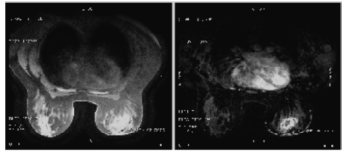
\includegraphics[width=6cm]{./img/contraste.png}
\centering
\end{figure}

Obtendo diversas imagens de contraste, é possível obter uma segmentação de pontos 3D, já utilizando uma filtragem a partirda classificação do algoritmo \textit{K-means algorithm}.
%
Um exemplo de nuvem de pontos com este filtro aplicado pode ser visualizado na Figura~\ref{fig:reconstrucao}.

\begin{figure}[htb]
\label{fig:reconstrucao}
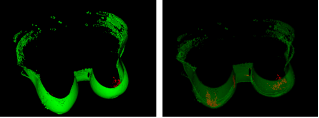
\includegraphics[width=6cm]{./img/reconstrucao.png}
\centering
\end{figure}

Pode ser visível como objeto final entregue ao médico que guiará o procedimento do paciente a visualização do objeto 3D descrito na Figura~\ref{fig:final}.

\begin{figure}[htb]
\label{fig:final}
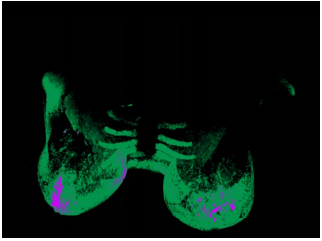
\includegraphics[width=6cm]{./img/final.png}
\centering
\end{figure}

A partir desta visualização, o médico poderá guiar sem falsos positivos ou eliminar problemáticas durante o procedimento de cura do câncer de mama, de forma mais barata e eficiente.

\section{Visualização de ossos da pélvis}

Segmentação de ossos é um método importante na tomografia guiada por computador~\cite{Yu2018May}.
%
Esta segumentação é utilizada para diagnosticos de danos na região pélvica, planejamento de operações e verificação do desempenho de tratamentos cirurgicos.
%
Esta segmentação pode ser realiada a partir da extração de pontos chaves baseado na diferança de pixels.
%
Utilizando este método, este diagnóstico pode ser realizado em aproximadamente 2 minutos por um computador, em média.

Para este método, é necessário um conjunto de imagens com fatiamnto da pélvis.
%
Isso pode ser obtido a partir de tomografia da região.
%
A entrada para este método computacional é um conjunto de imagens, a qual pode ser visualizado na Figura~\ref{fig:pelvis_contraste}.

\begin{figure}[htb]
\label{fig:pelvis_contraste}
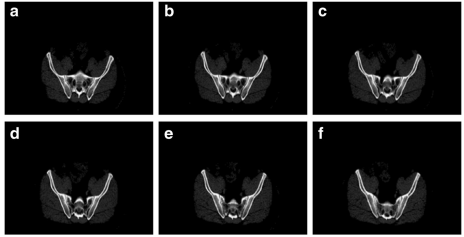
\includegraphics[width=6cm]{./img/pelvis_contraste.png}
\centering
\end{figure}

Entretando, se faz necessário o tratamento das imagens para limpar ruído obtido junto a tomografia.
%
Um exemplo do método de reomção de ruído pode ser visualizado na Figura~\ref{fig:pelvis_reconstrucao}.

\begin{figure}[htb]
\label{fig:pelvis_reconstrucao}
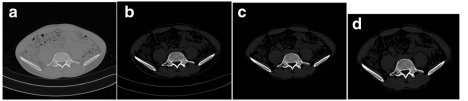
\includegraphics[width=6cm]{./img/pelvis_reconstrucao.png}
\centering
\end{figure}

O resultado final para planejamento médico será a reconstrução 3D e visualização do objeto para o médico que irá cuidar do procedimento de tratamento.
%
Nesse sentido, será entregue a Figura~\ref{fig:pelvis_final}.

\begin{figure}[htb]
\label{fig:pelvis_final}

\includegraphics[width=6cm]{./img/pelvis_final.png}
\centering
\end{figure}

Para este método, foi validado o seu uso em computadores pessoais com bom desempenho para uso clinico.
%
Entretanto, como este método depende do espaçamento de pontos chaves da tomografia, ele fica limitado a resolução da tomografia para a reconstrução 3D.
%
Caso seja obtido um número grande, se faz necessário métodos melhores para a reconstrução.
%
Por fim, pode-se utilizar a reconstrução utilizando GPU, descrito no inicio deste meta-artigo.

\section{Ultrassom 3D baseado em nuvem de pontos para tratamento de câncer de mama}

A fim de melhorar a visualização do procedimento médico de ultrassom, também pode-se utilizar a reconstrução de malhas 3D a partir de uma nuvem de pontos.
%
A implementação utiliza 150 imagens retiradas com ultrassom 2D para reconstrução 3D a fim de auxiliar no tratamento do câncer de mama~\cite{Michael2018May}.

Para este fim, foi utilizado os seguintes materiais:

\begin{enumerate}
  \item Scanner 3D
  \item Modelo de braço programável
  \item Monitoramento de braço
\end{enumerate}

A sua implantação final pode ser visualizada na Figura~\ref{fig:implantacao}.
%
Na mesma figura é possivel ver também um modelo do mesmo artefato desenvolvido em Autocad.

\begin{figure}[htb]
\label{fig:implantacao}
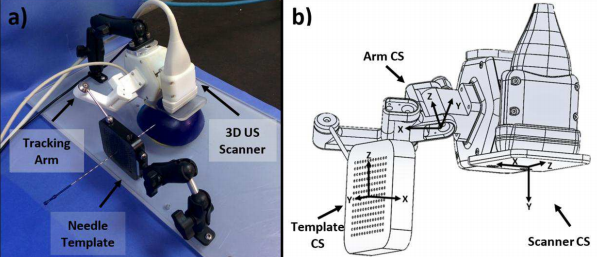
\includegraphics[width=6cm]{./img/implantacao.png}
\centering
\end{figure}

O resultado final entregue para exame pode ser visualizado na Figura~\ref{fig:scanner3d_final}.

\begin{figure}[htb]
\label{fig:scanner3d_final}
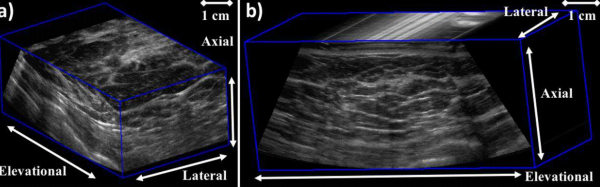
\includegraphics[width=6cm]{./img/scanner3d_final.png}
\centering
\end{figure}


\section{Laparoscópico para captura de nuvens de pontos}


A fim de evitar traumas e cortes em procedimentos cirurgicos, é comum utilizar câmeras a fim de realizar o procedimento sem expôr o objetivo a ambiente visível.
%
Entretanto, a utilização de câmeras permite somente a visualização de imagens 2D.
%
Por este motivo, pode-se utilizar um Laparascópico, uma tecnologia que permite a reconstrução da visualização 3D a partir de uma núvem de pontos junto a visualização tradicional 2D~\cite{Le2018May}.

Pode ser observado na Figura~\ref{fig:laparoscopico} a implementação de hardware do aparato médico.

\begin{figure}[htb]
\label{fig:laparoscopico}
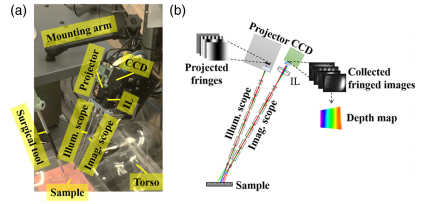
\includegraphics[width=6cm]{./img/laparoscopico.png}
\centering
\end{figure}

A fim de validar o seu funcionamento, se faz necessário sensores de alta precisão em curta distância.
%
Pode ser na Figura~\ref{fig:distancia} a intensidade de pontos obtidos da plotagem 3D pela distância de uma régua.


\begin{figure}[htb]
\label{fig:distancia}
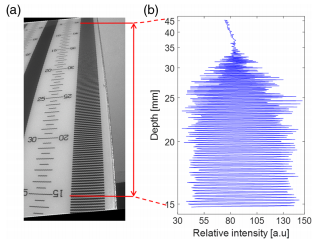
\includegraphics[width=6cm]{./img/distancia.png}
\centering
\end{figure}

Como objeto final entregue para o médico que realizará o procedimento médico é uma aplicação que exibirá uma nuvem de pontos para visualização 3D,
utilizando coloração para demonstrar um mapa de profundidade sobre a imagem original e a visão 2D tradicional.
%
Esta aplicação pode ser visualizada na Figura~\ref{fig:laparo_final}.

\begin{figure}[htb]
\label{fig:laparo_final}
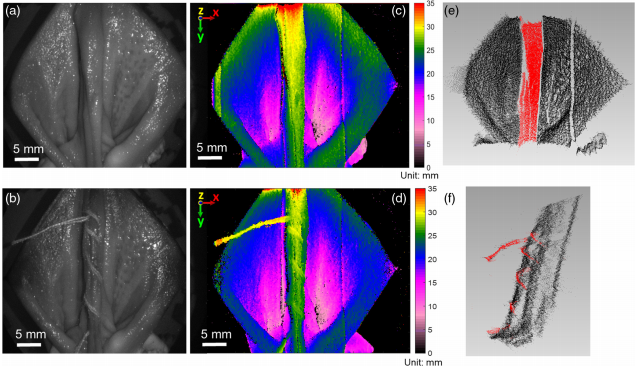
\includegraphics[width=6cm]{./img/laparo_final.png}
\centering
\end{figure}


Com o atual hardware foi obtido uma taxa de atualização de 1.72 imagens por segundo.
%
Entretanto, pode-se melhorar o seu desempenho caso seja alterado o sensor para escopos de precisão menor, em casos de exames menos minunciosos.

\section{Conclusão}

Dentre os artigos relatados, foi concluido um levantamento sobre o estado da arte da área.
%
Percebe-se a utilização em diversas áreas sobre tratamento de imagens para remoção de informação desnecessária e covnversão para nuvens de pontos, a fim de montar a topologia da nuvem em algoritmos para reconstrução de pontos.
%
Alguns temas abordaram desempenho, a fim de obter melhores métricas em casamento de imagens para gerar nuvens de pontos, outros abordam a utilização de tecnologia para o seu uso na medicina.
%
Entretanto, por não ser de um escopo conhecido pelo autor do atual trabalho, não pode-se avaliar a plena faculdade deste trabalho relacionado.

Um dos tópicos recorrentes é a detecção e auxilio de câncer de mama.
%
Este é o tópico mais abordado na busca de trabalhos relacionados ao tema.

Outro tema recorrente é a reconstrução a fim de auxiliar a visualização de ossos do corpo.
%
Em especial, da região pélvica, visto que contem várias sobrepossições dificultando uma análise concreta através de radiografias.
%
Estes objetos podem tanto auxiliar no planejamento e avaliação de procedimentos tanto quanto em projetos para protótipos médicos.

Por fim, percebe-se a ampla utilização de técnicas de reconstrução 3D utilizando nuvens de pontos a partir de imagens no ambiente hospitalar.
%
A fim de elaborar trabalhos futuros, o atual autor do trabalho tem interesse em melhorar sua proficiência nos algoritmos de reconstrução 3D a partir de nuvens de pontos,
%
visto que é amplamente utilizado em diversas áreas e possui um grande potencial acadêmico e comercial.



%%%%%%%%%%%%%%%%%%%%%%%%%%%%%%%%%%%%%%%%%%%%%%%%%%%%%%%%%%%%%%%%%%%%%%%%%%%%

\bibliographystyle{IEEEtran}
\bibliography{IEEEabrv,root}


\end{document}
